\subsection{Intergranular Fracture in \texorpdfstring{UO$_2$}{UO2}}

\subsectioncover

\begin{frame}{}
\vspace{-1.5em}
\begin{columns}
    \begin{column}{0.3\textwidth}
        \vspace{-2em}
        \begin{figure}[htb!]
            \centering
            \begin{subfigure}{\textwidth}
                \centering
                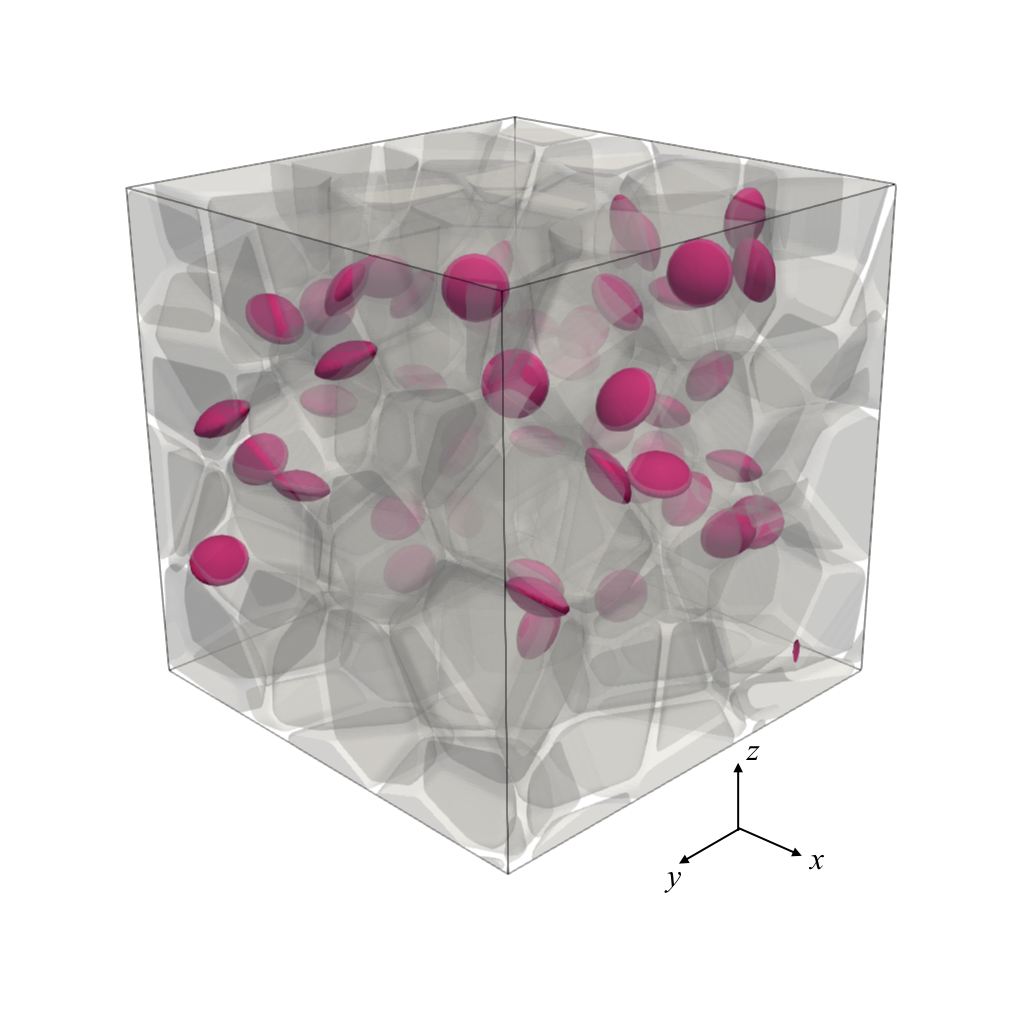
\includegraphics[width=0.5\textwidth]{past/figures/b50_ini_new.png}
            \end{subfigure}

            \begin{subfigure}{\textwidth}
                \centering
                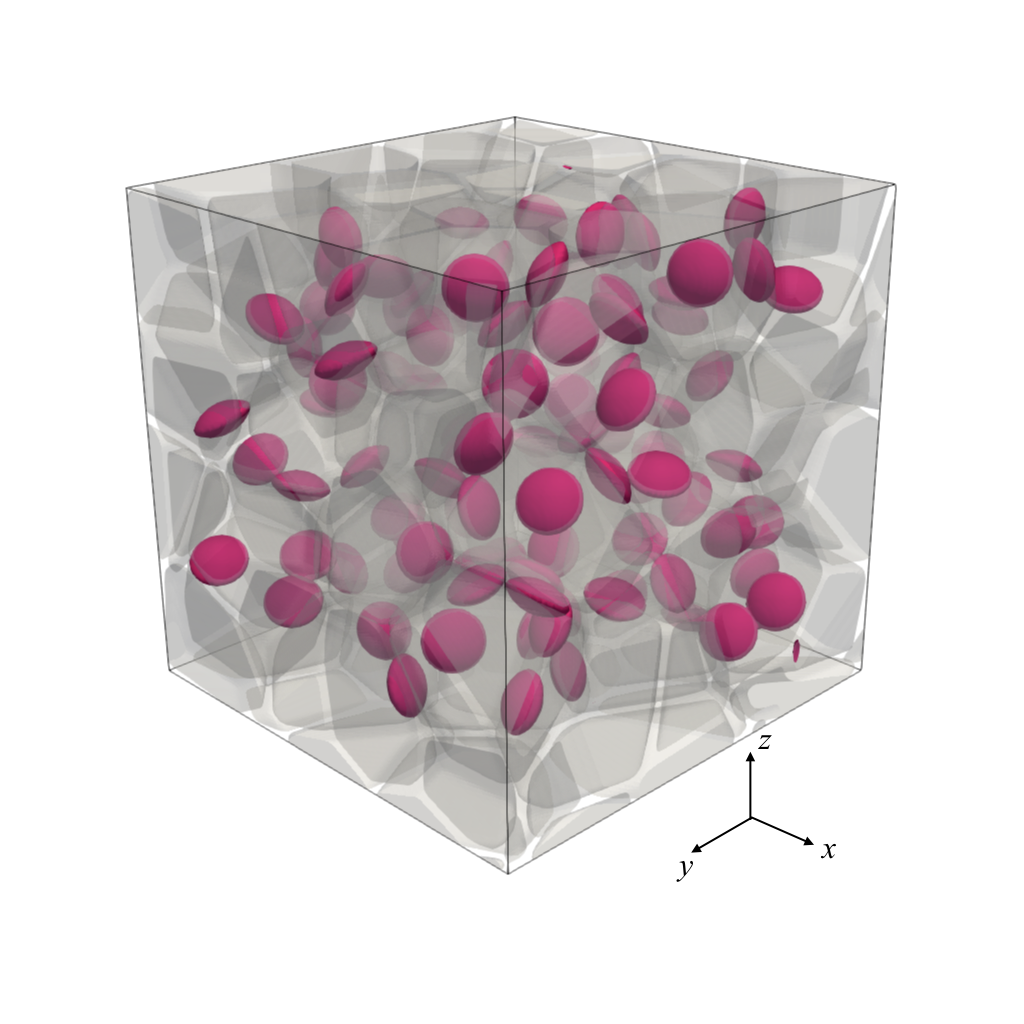
\includegraphics[width=0.5\textwidth]{past/figures/b100_ini_new.png}
            \end{subfigure}

            \begin{subfigure}{\textwidth}
                \centering
                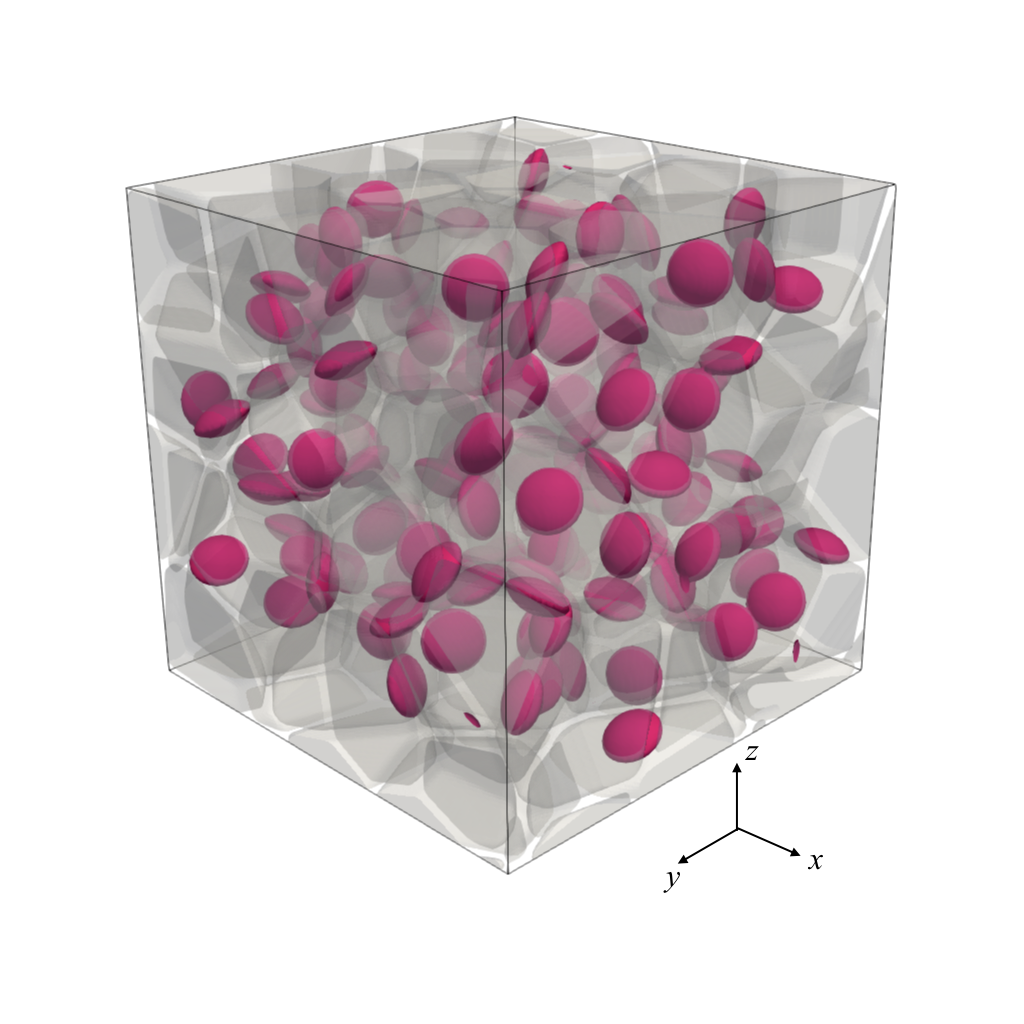
\includegraphics[width=0.5\textwidth]{past/figures/b150_ini_new.png}
            \end{subfigure}
        \end{figure}
        \vspace{-2em}
        \begin{exampleblock}{}
            See \texttt{intergranular.pdf} for details.
        \end{exampleblock}
    \end{column}
    \begin{column}{0.7\textwidth}
        \begin{itemize}
            \item A set of random close-packing (RCP) voronoi structures are realized by Maximal Poisson-disk Sampling (MPS).
            \item The polycrystalline microstructure is described by a set of non-conserved order variables $\{\phi_i\}$ in a diffuse manner.
            \item The microstructure follows from a phase-field grain growth model \cite{Moelans2008}.
            \item The grain boundaries are identified by $\sum_i \phi_i^2 \geqslant 0.75$.
            \item Gas bubbles are represented by another phase variable $\phi_0$ and are uniformly distributed along grain boundaries, overriding existing order variables. The effect of gas pressure inside bubbles is neglected.
            \pause
            \item A phase-field brittle fracture model is used.
            \item Grain boundaries have an arbitrarily high fracture toughness to facilitate intergranular fracture, i.e. $\Gc^\text{bnd} \gg \Gc^\text{grain}$.
            \pause
            \item \textcolor<4>{dukeroyal}{Numerical studies are performed to investigate the effect of bubble geometry, porosity and loading conditions on the fracture strength.}
        \end{itemize}
    \end{column}
\end{columns}
\end{frame}

\begin{frame}{}
\vspace{-1em}
\begin{columns}
    \begin{column}{0.33\textwidth}
        \contenttitle{Effect of bubble geometry} \\
        \begin{figure}[!htb]
    \centering
    \begin{subfigure}{\textwidth}
        \centering
        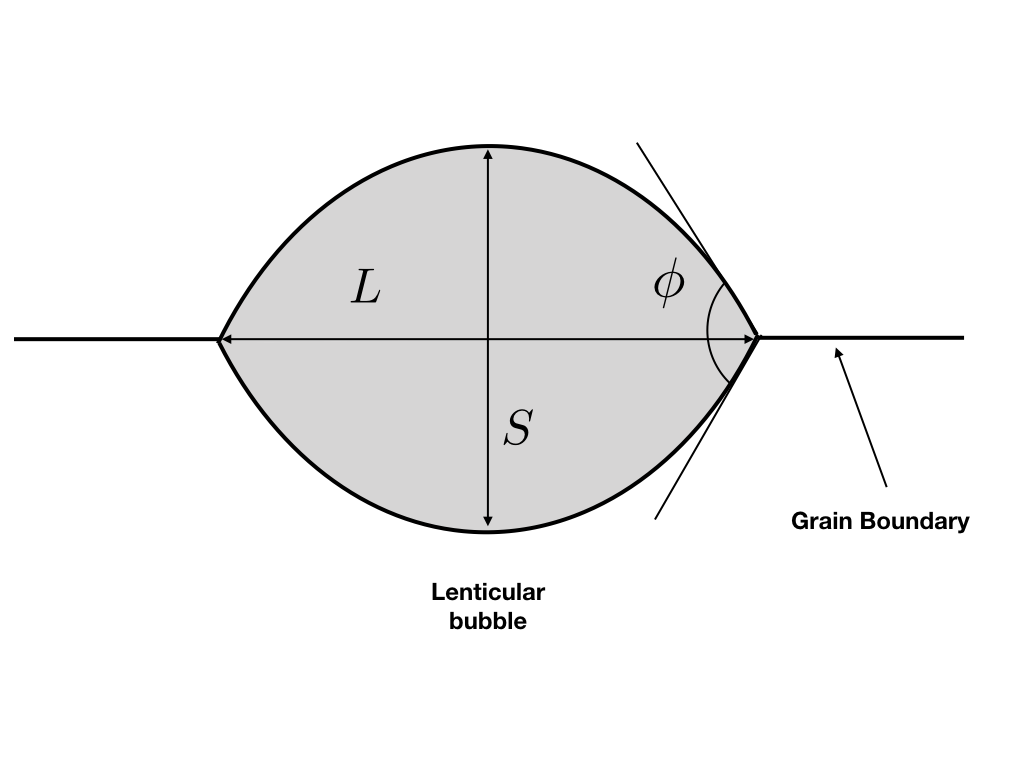
\includegraphics[width=0.6\textwidth]{past/figures/bub.png}
    \end{subfigure}

    \begin{subfigure}{\textwidth}
        \centering
        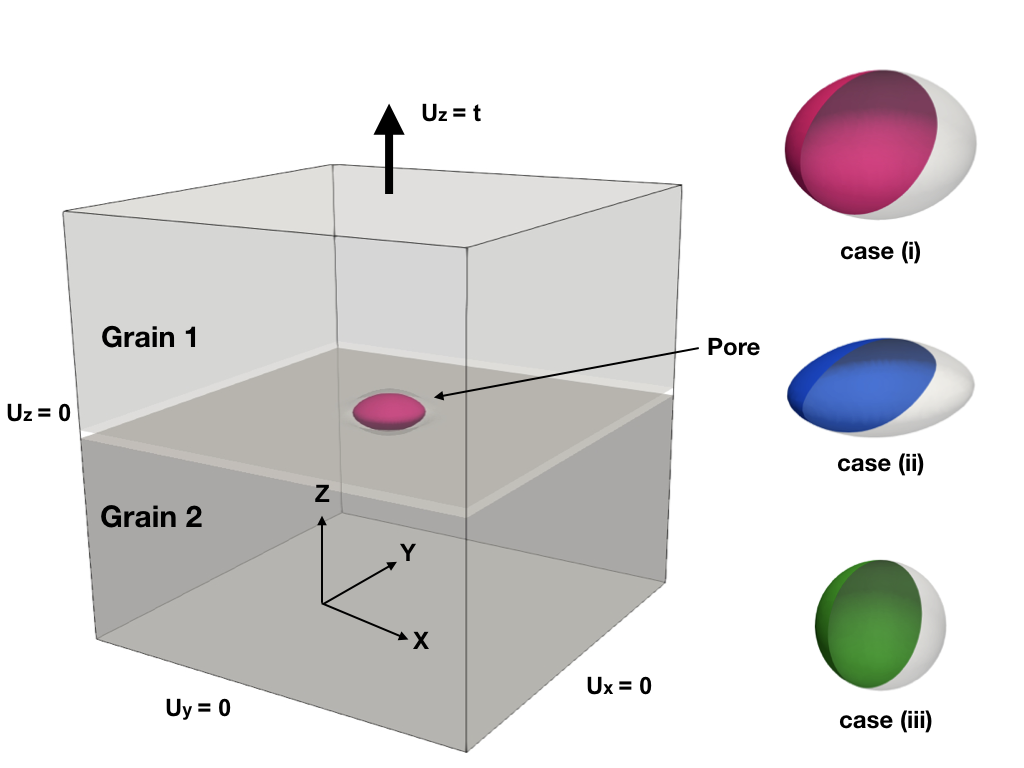
\includegraphics[width=0.6\textwidth]{past/figures/single_ini.png}
    \end{subfigure}

    \vspace{0.1in}
    \begin{tikzpicture}
        \begin{axis}[
            width=\textwidth,
            height=0.6\textwidth,
            ticks=none,
            xlabel=Strain,ylabel=Stress,
            xmin=0,
            xmax=0.006,
            ymin=0,
            ymax=700,
            every axis plot/.append style={line width=1pt}
        ]
            \addplot +[mark=none,color=red!60!black] table[x expr=\thisrowno{2}/40,y=ave_stress_top] {past/data/single_case1.csv};
            \addplot +[mark=none,color=blue!60!black] table[x expr=\thisrowno{2}/40,y=ave_stress_top] {past/data/single_case2.csv};
            \addplot +[mark=none,color=green!60!black] table[x expr=\thisrowno{2}/40,y=ave_stress_top] {past/data/single_case3.csv};
        \end{axis}
    \end{tikzpicture}
\end{figure}

    \end{column}
    \vrule{}
    \begin{column}{0.33\textwidth}
        \contenttitle{Effect of porosity} \\
        \begin{figure}[!htb]
    \centering
    \begin{subfigure}{0.35\textwidth}
        \centering
        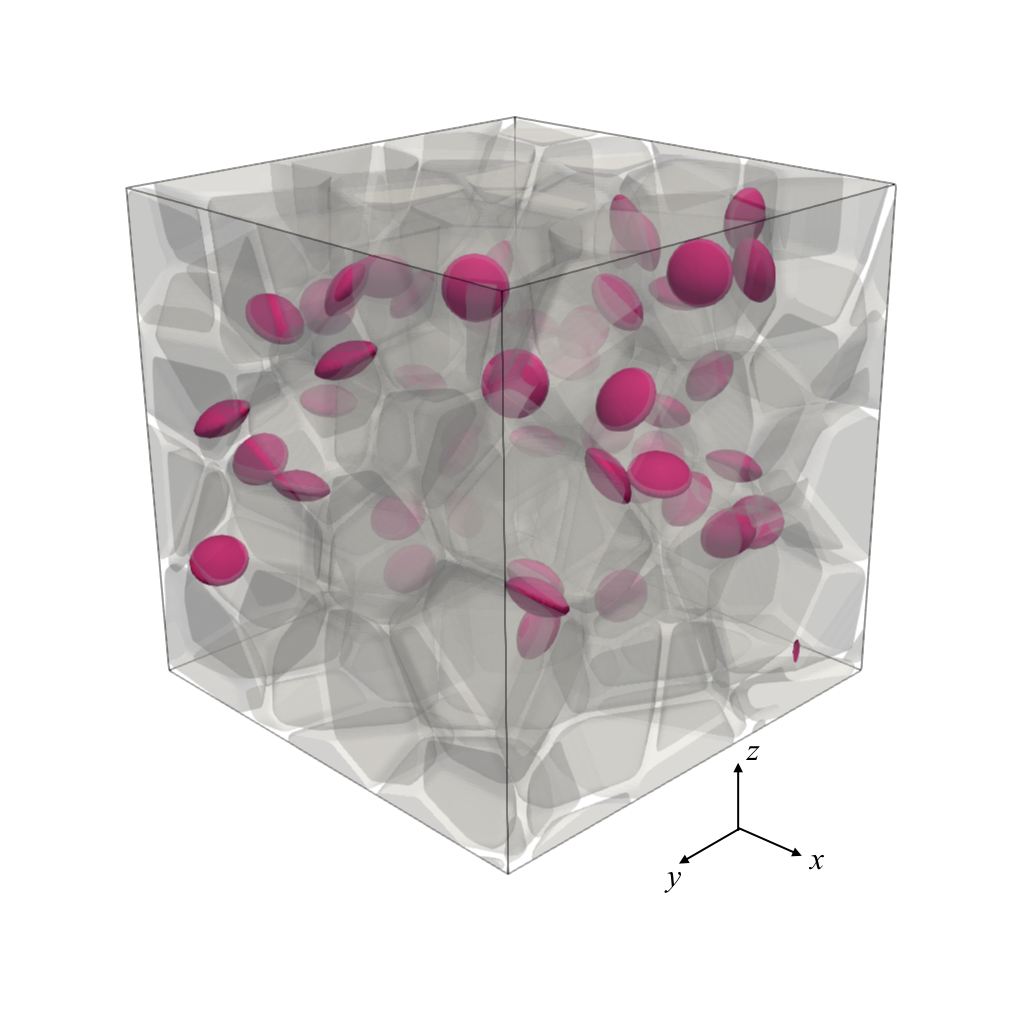
\includegraphics[width=\textwidth]{past/figures/b50_ini_new.png}
    \end{subfigure}
    \begin{subfigure}{0.35\textwidth}
        \centering
        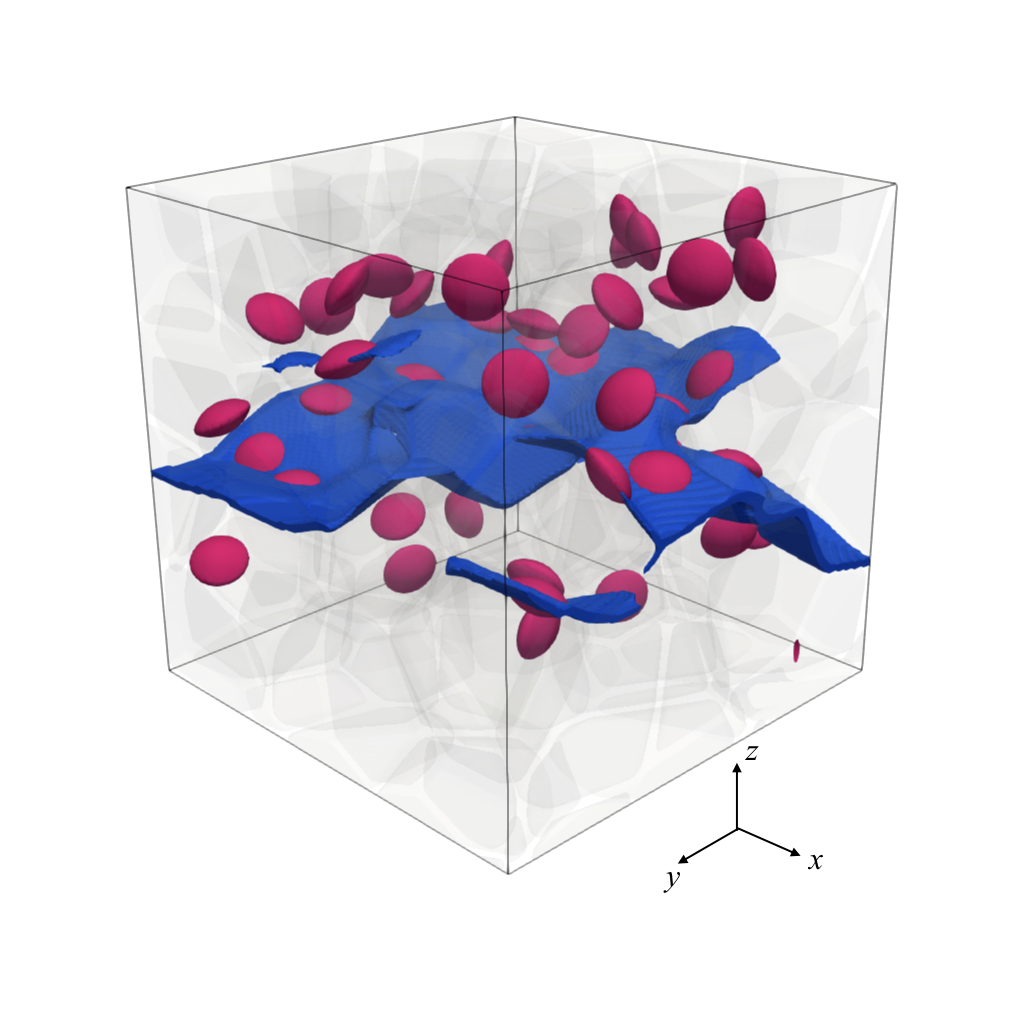
\includegraphics[width=\textwidth]{past/figures/b50_end.png}
    \end{subfigure}

    \vspace{-0.1in}
    \begin{subfigure}{0.35\textwidth}
        \centering
        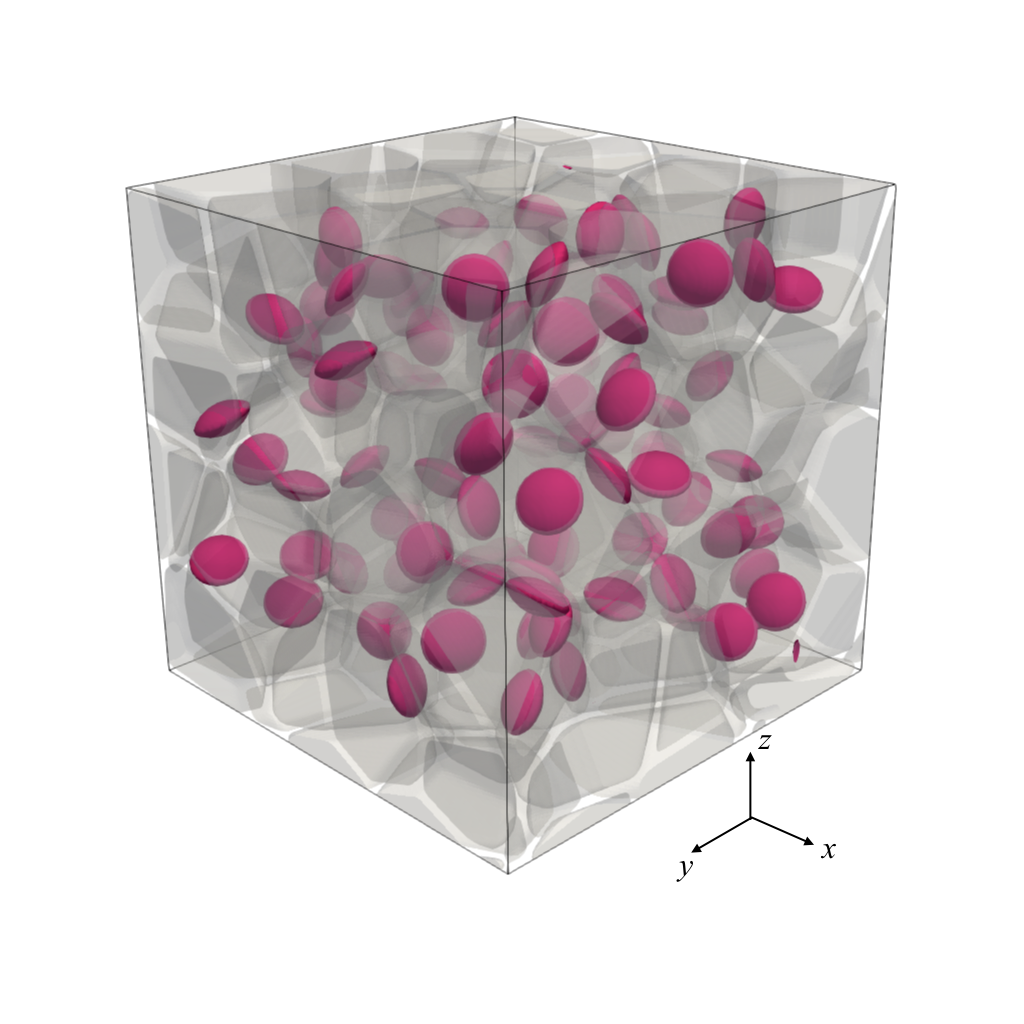
\includegraphics[width=\textwidth]{past/figures/b100_ini_new.png}
    \end{subfigure}
    \begin{subfigure}{0.35\textwidth}
        \centering
        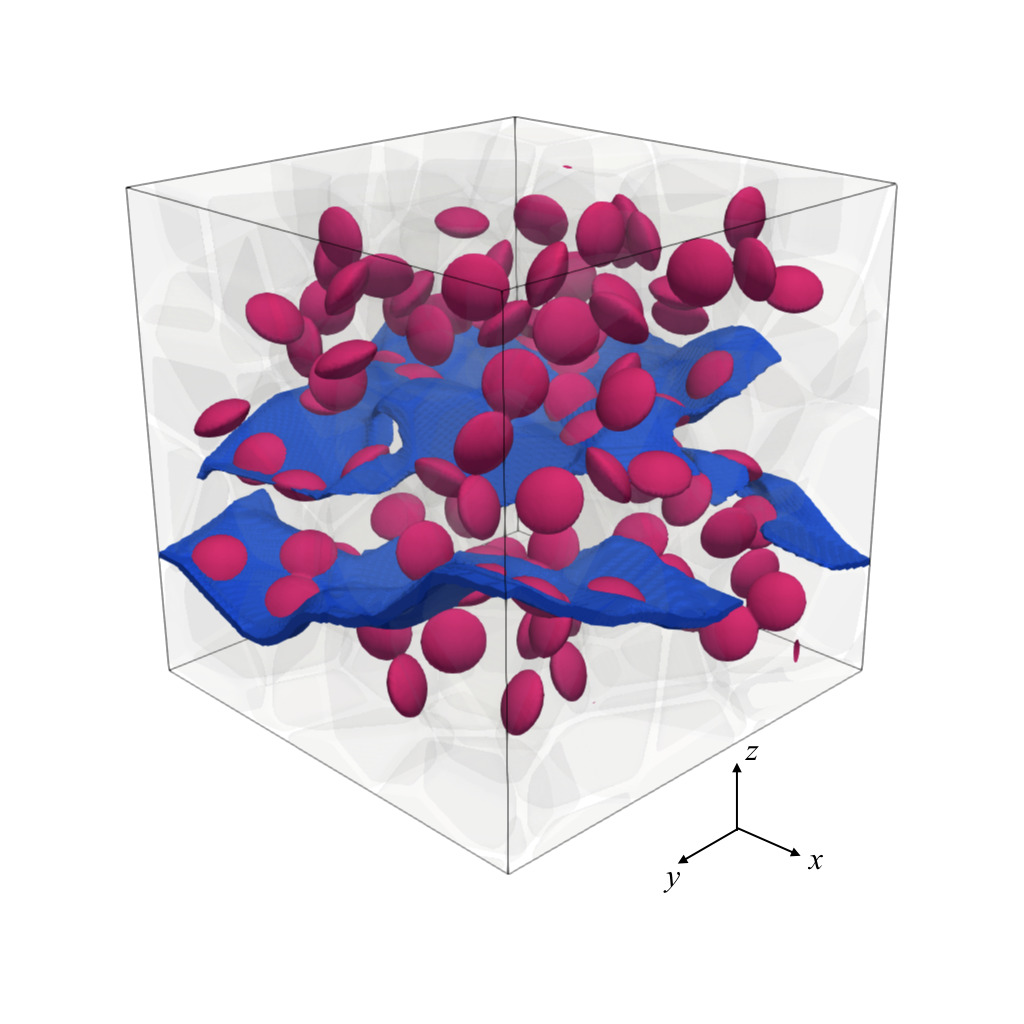
\includegraphics[width=\textwidth]{past/figures/b100_end.png}
    \end{subfigure}

    \vspace{-0.1in}
    \begin{subfigure}{0.35\textwidth}
        \centering
        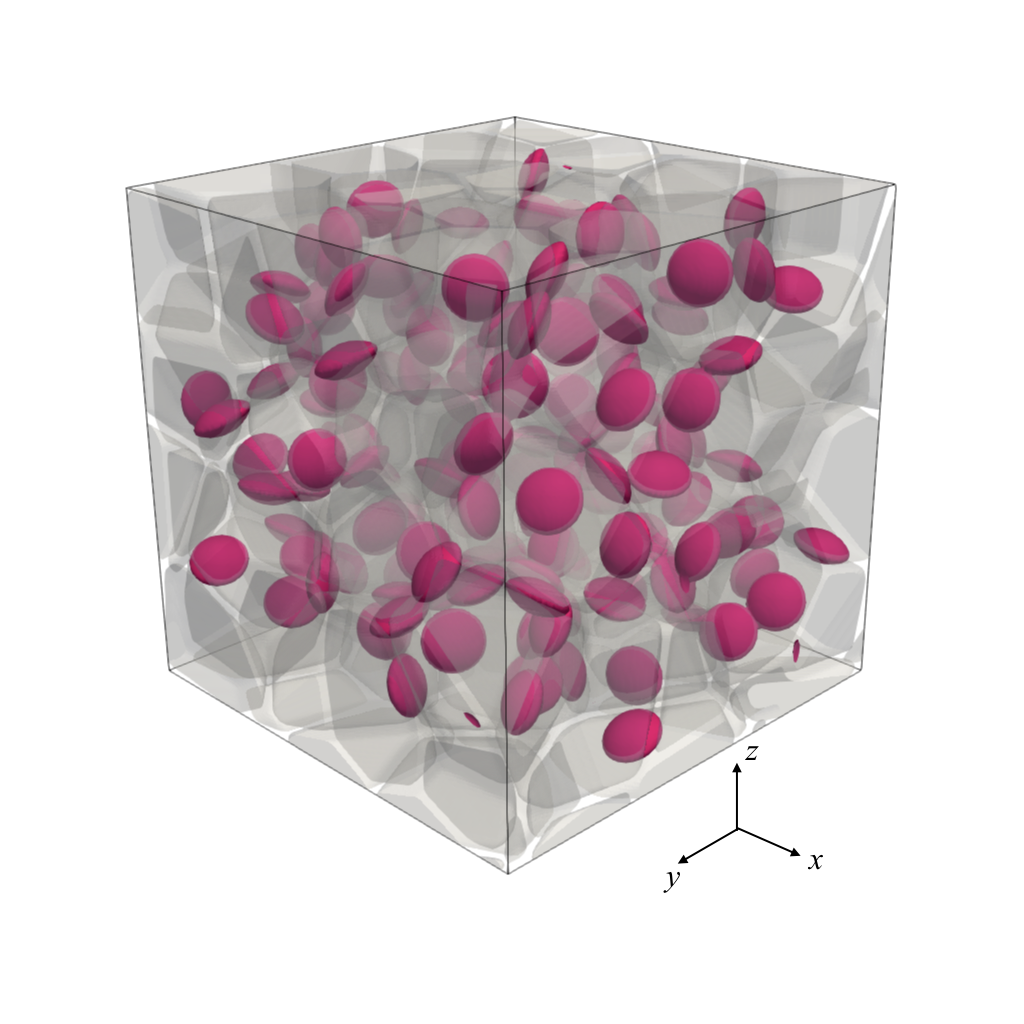
\includegraphics[width=\textwidth]{past/figures/b150_ini_new.png}
    \end{subfigure}
    \begin{subfigure}{0.35\textwidth}
        \centering
        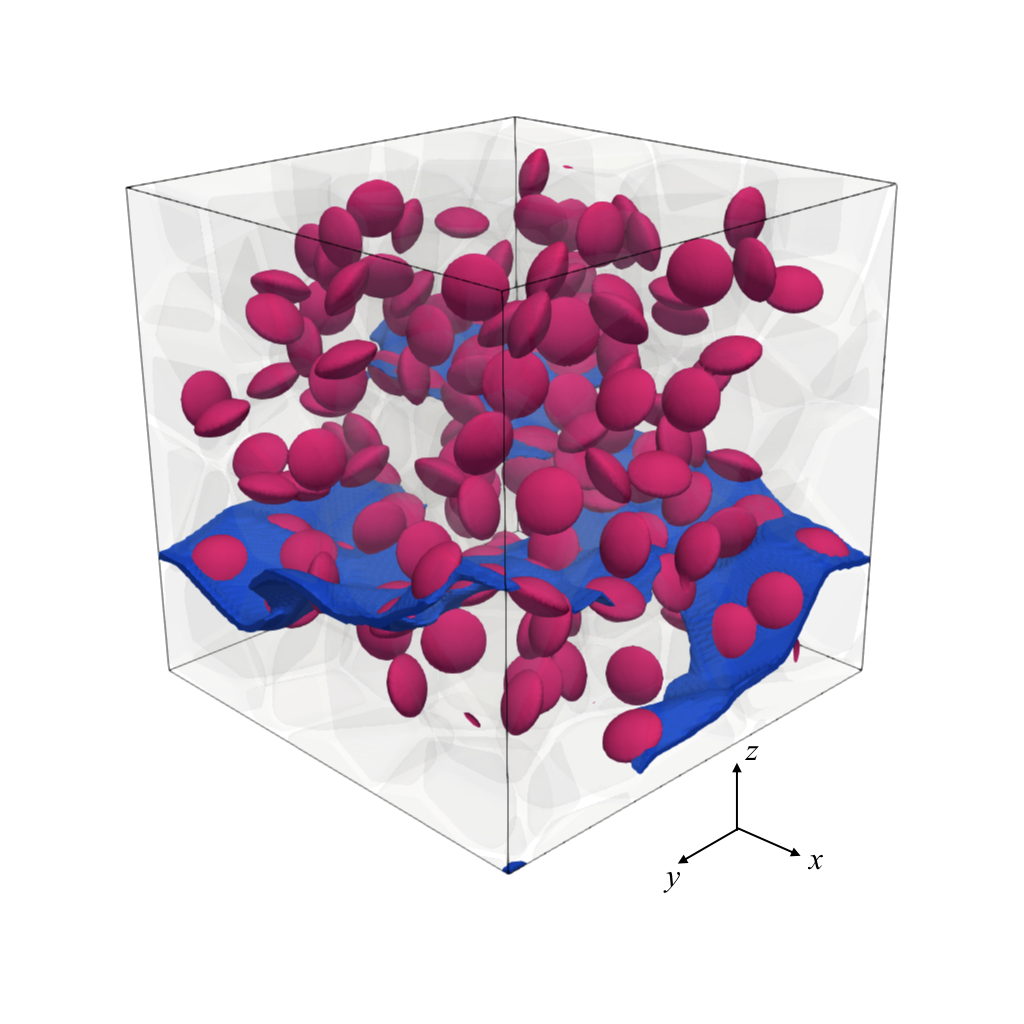
\includegraphics[width=\textwidth]{past/figures/b150_end.png}
    \end{subfigure}

    \begin{tikzpicture}
        \begin{axis}[
            width=\textwidth,
            height=0.6\textwidth,
            ticks=none,
            xlabel=Strain,ylabel=Stress,
            xmin=0,
            xmax=0.0025,
            ymin=0,
            ymax=700,
            every axis plot/.append style={line width=1pt}
        ]
            \addplot +[mark=none,color=black,solid] table[x expr=\thisrowno{2}/40,y=ave_stress_top] {past/data/b50_out.csv};
            \addplot +[mark=none,color=black,dashed] table[x expr=\thisrowno{2}/40,y=ave_stress_top] {past/data/b100_out.csv};
            \addplot +[mark=none,color=black,dotted] table[x expr=\thisrowno{2}/40,y=ave_stress_top] {past/data/b150_out.csv};
        \end{axis}
    \end{tikzpicture}
\end{figure}

    \end{column}
    \vrule{}
    \begin{column}{0.33\textwidth}
        \contenttitle{Effect of loading direction} \\
        \begin{figure}[!htb]
    \centering
    \begin{subfigure}{0.35\textwidth}
        \centering
        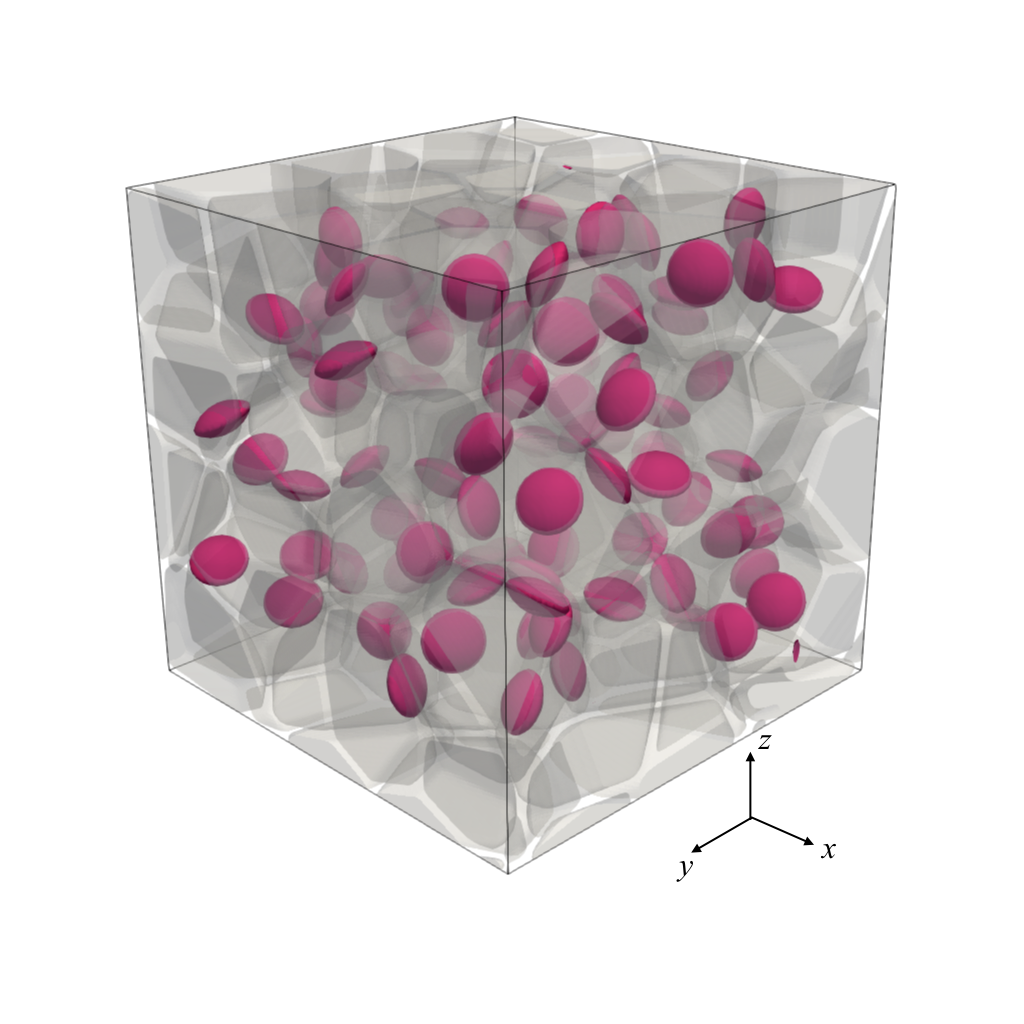
\includegraphics[width=\textwidth]{past/figures/b100_ini_new.png}
    \end{subfigure}
    \begin{subfigure}{0.35\textwidth}
        \centering
        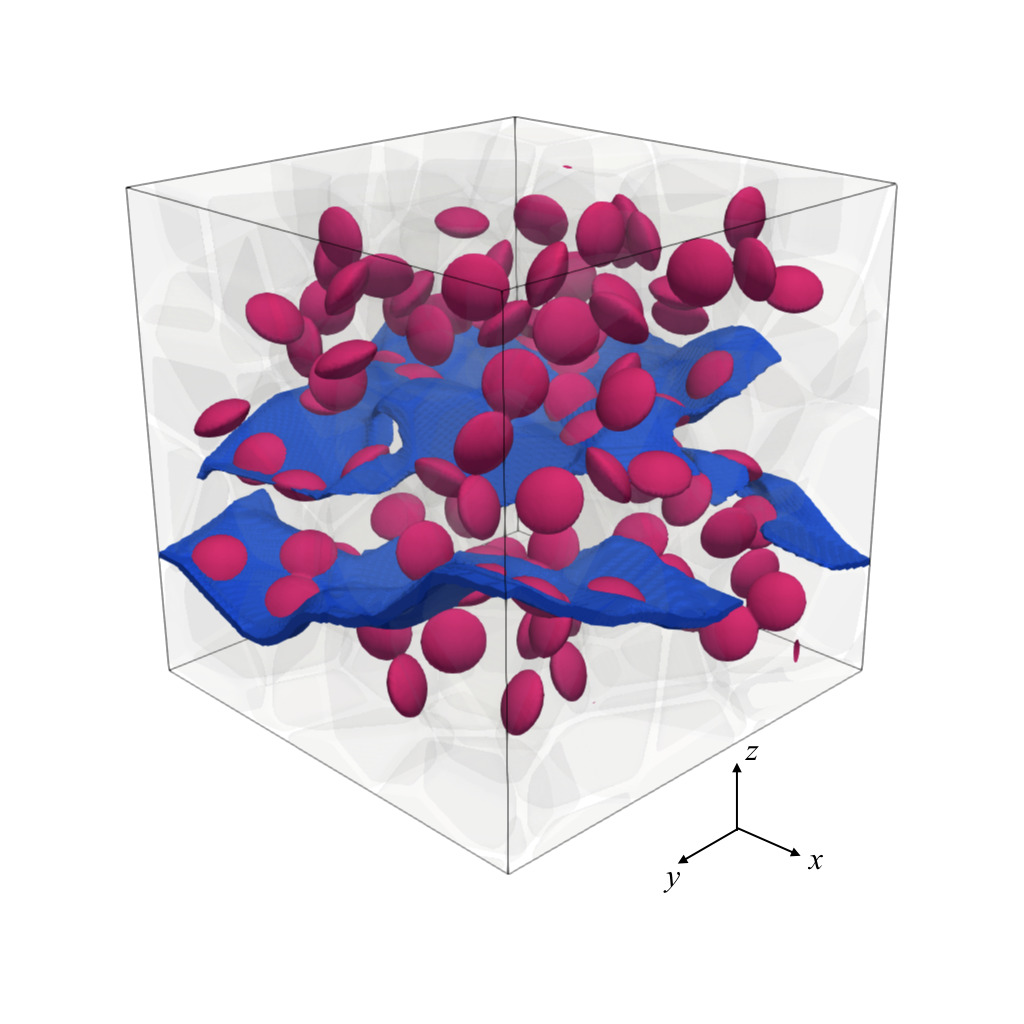
\includegraphics[width=\textwidth]{past/figures/b100_end.png}
    \end{subfigure}

    \vspace{-0.1in}
    \begin{subfigure}{0.35\textwidth}
        \centering
        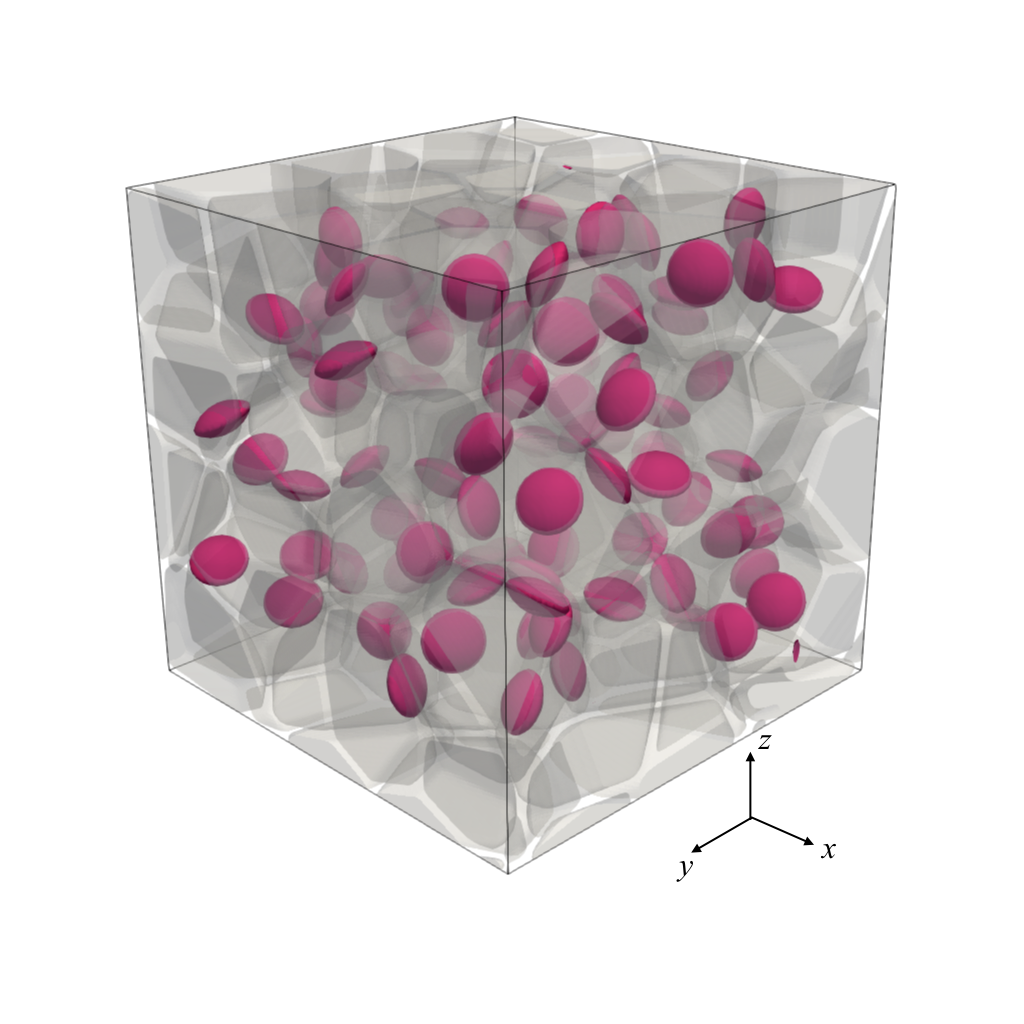
\includegraphics[width=\textwidth]{past/figures/b100_ini_new.png}
    \end{subfigure}
    \begin{subfigure}{0.35\textwidth}
        \centering
        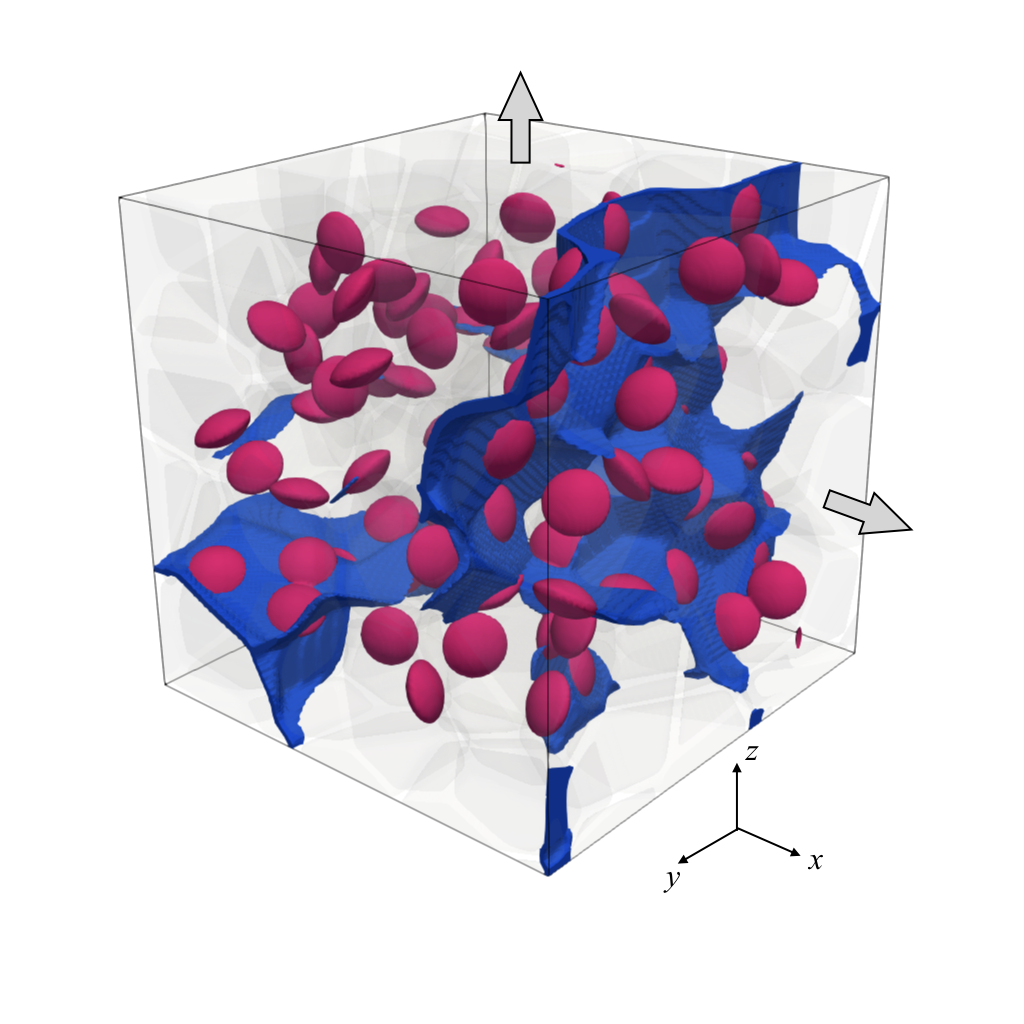
\includegraphics[width=\textwidth]{past/figures/b100_end_yz.png}
    \end{subfigure}

    \vspace{-0.1in}
    \begin{subfigure}{0.35\textwidth}
        \centering
        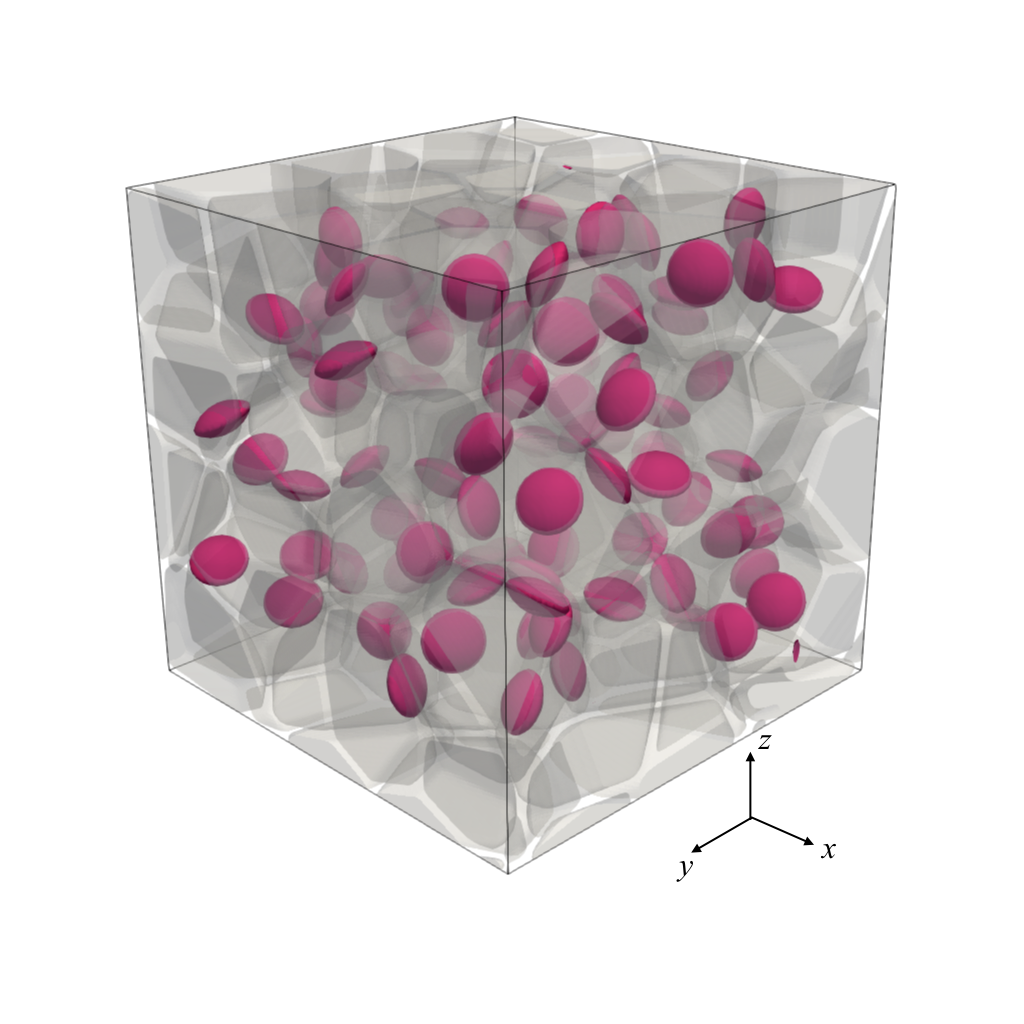
\includegraphics[width=\textwidth]{past/figures/b100_ini_new.png}
    \end{subfigure}
    \begin{subfigure}{0.35\textwidth}
        \centering
        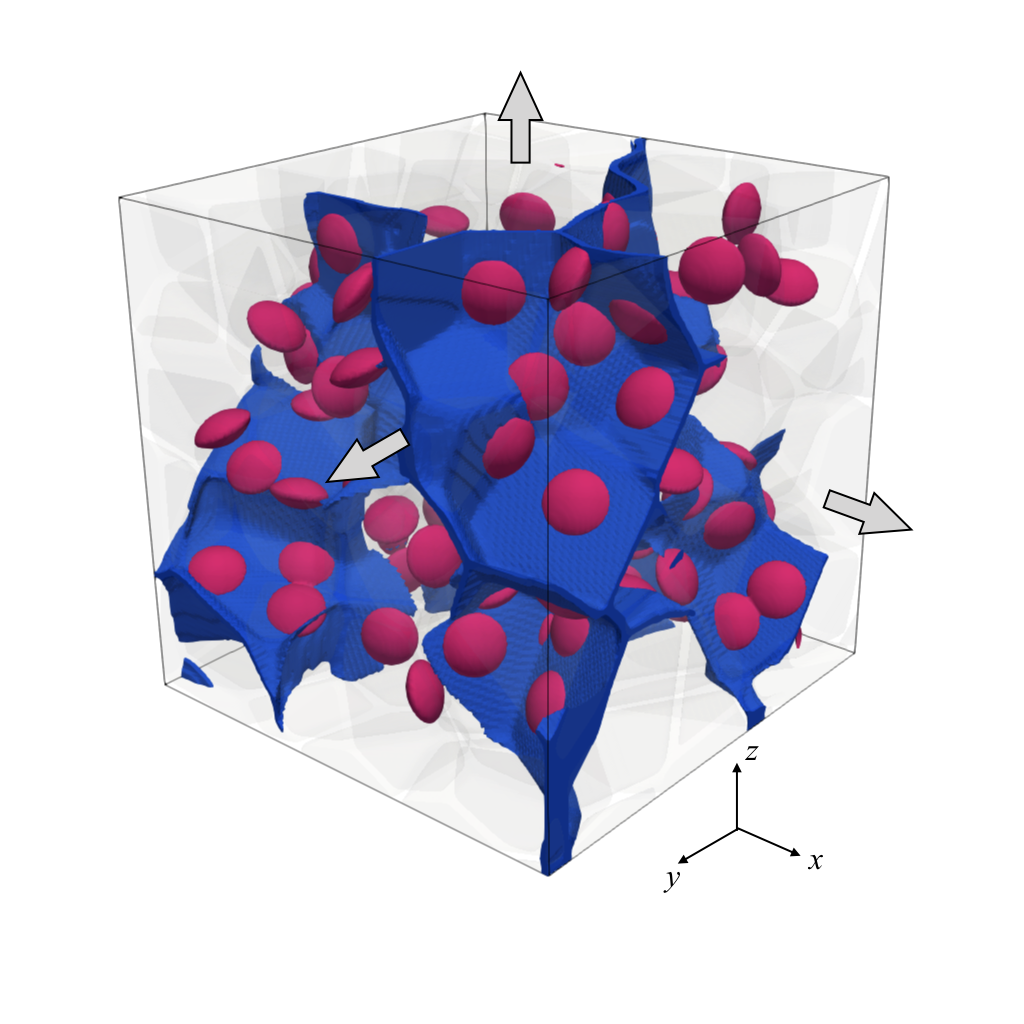
\includegraphics[width=\textwidth]{past/figures/b100_end_xyz.png}
    \end{subfigure}

    \begin{tikzpicture}
        \begin{axis}[
            width=\textwidth,
            height=0.6\textwidth,
            ticks=none,
            xlabel=Strain,ylabel=Stress,
            xmin=0,
            xmax=0.0025,
            ymin=0,
            ymax=700,
            every axis plot/.append style={line width=1pt}
        ]
            \addplot +[mark=none,color=black,solid] table[x expr=\thisrowno{2}/40,y=ave_stress_top] {past/data/b100_y.csv};
            \addplot +[mark=none,color=black,dashed] table[x expr=\thisrowno{5}/40,y=ave_stress_top] {past/data/b100_yz.csv};
            \addplot +[mark=none,color=black,dotted] table[x expr=\thisrowno{5}/40,y=ave_stress_top] {past/data/b100_xyz.csv};
        \end{axis}
    \end{tikzpicture}
\end{figure}

    \end{column}
\end{columns}
\end{frame}
